\documentclass[11pt,a4paper]{article}

\usepackage[utf8]{inputenc}
\usepackage[T1]{fontenc}
\usepackage[spanish,es-tabla]{babel}
\usepackage{lmodern}
\usepackage[margin=2.5cm]{geometry}
\usepackage{graphicx}
\usepackage{booktabs}
\usepackage{tabularx}
\usepackage{array}
\usepackage{amsmath}
\usepackage{enumitem}
\usepackage{caption}
\usepackage{float}
\usepackage{needspace}
\usepackage{tikz}
\usetikzlibrary{arrows.meta,positioning,babel}
\usepackage{pgfgantt}
\usepackage[most]{tcolorbox}
\definecolor{radar}{RGB}{37,99,235}
\definecolor{agua}{RGB}{16,150,120}
\usepackage[hidelinks]{hyperref}

\graphicspath{{figuras/}}
\newcolumntype{L}{>{\raggedright\arraybackslash}X}
\setlength{\parskip}{0.5em}
\setlength{\parindent}{0pt}
\renewcommand{\arraystretch}{1.3}
\setlist{itemsep=2pt, topsep=2pt}

% ------------------------------------------------------
% Etiquetas de estado
% ------------------------------------------------------
\newcommand{\chip}[2]{\tikz[baseline=(c.base)]\node[fill=#1, text=white,
    rounded corners=2pt, inner sep=2.5pt, font=\scriptsize\bfseries\sffamily] (c) {#2};}
\newcommand{\REAL}{\chip{agua}{REALIZADO}}
\newcommand{\SEG}{\chip{radar}{2.º PARCIAL}}
\newcommand{\FUERA}{\chip{gray}{FUERA DE ALCANCE}}

% Barra de puntaje (0 a 5)
\newcommand{\barra}[1]{\tikz[baseline=-0.5ex]{
    \fill[gray!20] (0,-0.12) rectangle (2,0.12);
    \fill[radar] (0,-0.12) rectangle (#1*0.4,0.12);}}

% Observación del evaluador
\newtcolorbox{debilidad}{enhanced, colback=gray!7, colframe=gray!45,
    boxrule=0.5pt, arc=3pt, left=7pt, right=7pt, top=4pt, bottom=4pt,
    fontupper=\itshape\small}

% Encabezado de cada punto: criterio, puntaje, estados
\newcommand{\punto}[3]{%
    \needspace{12\baselineskip}
    \section{#1}
    \textbf{Puntaje: #2/5} \quad #3\par}

\begin{document}

% ======================================================
% PORTADA
% ======================================================
\begin{titlepage}
    \centering
    {\large Universidad Nacional de Asunción\par}
    {\large Facultad de Ingeniería\par}
    {\large Carrera de Ingeniería Mecatrónica\par}
    \vspace{1.2cm}
    
\includegraphics[width=0.32\textwidth]{logo_fiuna.png}\par
    \vspace{1.2cm}
    {\Large Proyecto 4\par}
    \vspace{1.2cm}
    {\LARGE\bfseries Sistema de adquisición y monitoreo\\de nivel de agua\par}
    \vspace{0.6cm}
    {\Large Respuesta a la evaluación detallada\\del primer parcial\par}
    \vfill
    \begin{flushleft}
        \textbf{Profesores:}\\
        Prof. Ing. Federico Gaona, MSc.\\
        Prof. Ing. Esteban Fretes\\[1em]
        \textbf{Alumnos:}\\
        \begin{tabular}{@{}ll}
            Héctor Dejesús Velázquez Ojeda   & 5.011.166 \\
            Mathias Ramón Aguilar DelValle   & 4.970.804 \\
            Mauricio Iván Tullo Estigarribia & 3.782.101 \\
        \end{tabular}
    \end{flushleft}
    \vspace{1cm}
    {\large San Lorenzo, Paraguay\par}
    {\large 2026\par}
\end{titlepage}

% ======================================================
% RESUMEN
% ======================================================
\section*{Resumen}

La evaluación detallada del primer parcial señaló diez aspectos a mejorar, uno
por criterio de la rúbrica. Para cada uno indicamos qué ya está resuelto, qué
presentaremos en el segundo parcial (16 de noviembre) y qué queda fuera del
alcance del proyecto, con su justificación.

Los cambios principales son el reemplazo del sensor ultrasónico por un
\textbf{radar de 80 GHz} que además mide la velocidad superficial del agua, una
\textbf{trama de datos con identificador y estado}, una \textbf{web propia}
para mostrar los datos y un \textbf{plan de ensayos en banco de laboratorio}
con resultados medibles. Todas las pruebas se harán en laboratorio, porque la
instalación en el arroyo depende del Departamento de Mecánica y Energía.

\begin{center}
    \REAL\ ya resuelto \qquad
    \SEG\ se presenta el 16/11 \qquad
    \FUERA\ justificado
\end{center}

\begin{table}[H]
    \centering
    \caption{Los diez criterios evaluados y su estado.}
    \begin{tabular}{rl c c l}
        \toprule
        & \textbf{Criterio} & \textbf{Puntaje} & & \textbf{Estado} \\
        \midrule
        1  & Problema y relevancia         & 4   & \barra{4}   & \SEG \\
        2  & Objetivos y alcance           & 3   & \barra{3}   & \REAL \\
        3  & Metodología                   & 3,5 & \barra{3.5} & \SEG\ \FUERA \\
        4  & Arquitectura y requisitos     & 4   & \barra{4}   & \REAL\ \SEG \\
        5  & Diseño electrónico            & 4   & \barra{4}   & \SEG \\
        6  & Diseño mecánico/estructural   & 3,5 & \barra{3.5} & \SEG\ \FUERA \\
        7  & Interfaz de usuario           & 4   & \barra{4}   & \SEG\ \FUERA \\
        8  & Validación y seguridad        & 2,5 & \barra{2.5} & \SEG\ \FUERA \\
        9  & Bibliografía y aporte propio  & 3,5 & \barra{3.5} & \SEG \\
        10 & Viabilidad y documentación    & 3,5 & \barra{3.5} & \SEG\ \FUERA \\
        \bottomrule
    \end{tabular}
\end{table}

\newpage

% ======================================================
% 1. PROBLEMA Y RELEVANCIA
% ======================================================
\punto{Problema y relevancia}{4}{\SEG}

\begin{debilidad}
No cuantifica pérdidas de datos, incertidumbre ni limitaciones de la solución
previa.
\end{debilidad}

\textbf{Respuesta.}
\begin{itemize}
    \item \textbf{Usuario:} la ciudadanía. Los datos son \emph{abiertos} y el
        fin del proyecto es que el nivel y su predicción lleguen a la sociedad
        a través de una aplicación.
    \item \textbf{Pérdidas de datos (línea de base):} la estación de P3 lleva
        unos 9 meses enviando datos. Tenemos acceso total a ellos, así que
        calcularemos la \textbf{disponibilidad} (datos recibidos frente a
        esperados) y la cantidad y duración de los huecos.
    \item \textbf{Incertidumbre:} el sensor ultrasónico se reemplaza por un
        radar de $\pm$3 mm (según la ficha). Su error real se mide en banco
        (punto~\ref{sec:validacion}).
\end{itemize}

\begin{figure}[H]
    \centering
    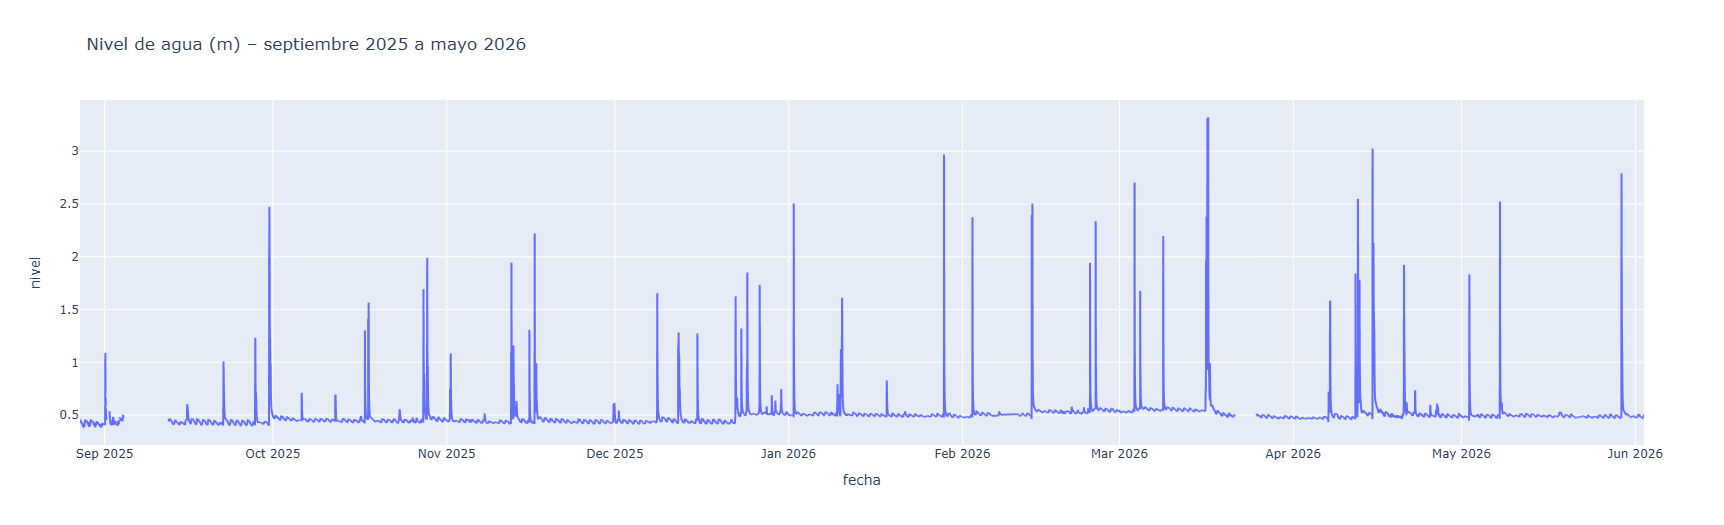
\includegraphics[width=\textwidth]{datos_p3.png}
    \caption{Datos de la estación de P3 (septiembre 2025 a mayo 2026). Los
    huecos visibles, por ejemplo en septiembre y a fines de marzo, son los
    que vamos a cuantificar.}
\end{figure}

% ======================================================
% 2. OBJETIVOS Y ALCANCE
% ======================================================
\punto{Objetivos y alcance}{3}{\REAL}

\begin{debilidad}
Quince objetivos mezclan actividades y resultados; faltan metas de exactitud y
disponibilidad y un objetivo explícito de interfaz.
\end{debilidad}

\textbf{Respuesta.} Ya lo resolvimos en el informe de puntos de mejora: los 15
objetivos pasaron a 5, uno por área, con un criterio de aceptación medible.
Ahora sumamos la meta de \textbf{disponibilidad} que faltaba.

\begin{table}[H]
    \centering
    \caption{Objetivos específicos y criterios de aceptación.}
    \begin{tabularx}{\textwidth}{>{\raggedright\arraybackslash}p{2.4cm}LL}
        \toprule
        \textbf{Área} & \textbf{Objetivo} & \textbf{Criterio de aceptación} \\
        \midrule
        Electrónica & Integrar radar, RTC, microSD y módem, con consumo y
            autonomía conocidos. & Consumo medido por módulo y autonomía
            medida con la UPS. \\
        Firmware & Enviar los datos sin perderlos ante cortes (Store and
            Forward con ID). & 0 perdidos y 0 duplicados en $\geq$ 10 cortes;
            \textbf{disponibilidad $\geq$ 95\,\%} en 7 días. \\
        Montaje & Montar el radar con su kit en un banco de laboratorio. &
            Antena nivelada y haz libre de obstáculos. \\
        Interfaz & Web con históricos, antigüedad del dato, estado del sensor
            y alarma. & Capturas con dato válido, viejo y en falla. \\
        Validación & Medir la exactitud del nivel en el banco. & Error
            $\leq \pm$10 mm frente a cinta métrica. \\
        \bottomrule
    \end{tabularx}
\end{table}

% ======================================================
% 3. METODOLOGIA
% ======================================================
\punto{Metodología}{3,5}{\SEG\ \FUERA}

\begin{debilidad}
No explicita comparación de alternativas ni protocolo experimental completo;
riesgo de confundir implementación con método.
\end{debilidad}

\textbf{Respuesta.}
\begin{itemize}
    \item \SEG\ \textbf{Comparación de alternativas:} a fines de septiembre
        comparamos sensores de toda la gama, del más económico al más caro,
        por calidad y precio. Elegimos el radar FM02B porque, además del nivel,
        mide la \textbf{velocidad superficial del agua}, un dato más para la
        predicción. La tabla comparativa se incluye en el segundo parcial.
    \item \SEG\ \textbf{Protocolo experimental:} cada ensayo indicará qué se
        mide, con qué instrumento, cuántas repeticiones y qué umbral se usa
        (punto~\ref{sec:validacion}).
    \item \FUERA\ \textbf{Piloto en el arroyo:} la instalación en el sitio
        depende del Departamento de Mecánica y Energía. Todas las pruebas se
        hacen en un banco de laboratorio que simula la instalación.
\end{itemize}

% ======================================================
% 4. ARQUITECTURA Y REQUISITOS
% ======================================================
\punto{Arquitectura y requisitos}{4}{\REAL\ \SEG}

\begin{debilidad}
El nivel H$-$d exige datum estable; nivel $-1$ mezcla error con dato. El ajuste
RTC +3 h carece de convención horaria suficientemente clara.
\end{debilidad}

\textbf{Respuesta.}
\begin{itemize}
    \item \REAL\ \textbf{Convención horaria:} Paraguay usa horario fijo
        UTC$-$3, sin cambio estacional. El RTC guarda la hora local y el
        firmware suma 3 h, así que \textbf{todo dato enviado está en UTC}
        (tiempo epoch). Se eligió así para no depender de cambios de horario.
    \item \SEG\ \textbf{Contrato de datos:} el firmware se reescribe para el
        radar, y con eso cambia la trama. Cada dato lleva un \textbf{id}
        secuencial y un campo de \textbf{estado}, así que una falla ya no se
        envía como el valor $-1$. Tenemos acceso al servidor para adaptarlo.
    \item \textbf{Datum:} la altura de referencia se fija al instalar. En el
        banco es la altura conocida del sensor.
\end{itemize}

\begin{figure}[H]
    \centering
    % Trama actual (P3) frente a la trama propuesta para el 2.o parcial
\begin{tikzpicture}[
    campo/.style={draw=gray!70, fill=white, minimum height=0.75cm, inner sep=4pt, font=\small\ttfamily},
    nuevo/.style={campo, draw=radar, fill=radar!10},
    nota/.style={font=\footnotesize, text=gray!60!black, align=center}
]
    % Trama actual
    \node[anchor=west, font=\small\bfseries] at (0,0.9) {Actual (P3)};
    \node[campo, anchor=west] (a1) at (0,0) {d=};
    \node[campo, right=0pt of a1] (a2) {epoch};
    \node[campo, right=0pt of a2, draw=red!70, fill=red!8] (a3) {valor};
    \node[nota, below=3pt of a3] {si el sensor falla\\se envía $-1$};

    % Trama nueva
    \node[anchor=west, font=\small\bfseries] at (0,-2.0) {Propuesta (2.\textsuperscript{o} parcial)};
    \node[campo, anchor=west] (b1) at (0,-2.9) {d=};
    \node[campo, right=0pt of b1] (b2) {epoch UTC};
    \node[nuevo, right=0pt of b2] (b3) {id};
    \node[campo, right=0pt of b3] (b4) {distancia};
    \node[nuevo, right=0pt of b4] (b5) {velocidad};
    \node[nuevo, right=0pt of b5] (b6) {estado};
    \node[nota, below=3pt of b3] {secuencial:\\detecta perdidos\\y duplicados};
    \node[nota, below=3pt of b5] {dato nuevo\\del radar};
    \node[nota, right=6pt of b6] {OK / FALLA\\(separado\\del dato)};
\end{tikzpicture}

    \caption{Trama enviada al servidor: actual y propuesta.}
\end{figure}

% ======================================================
% 5. DISENO ELECTRONICO
% ======================================================
\punto{Diseño electrónico}{4}{\SEG}

\begin{debilidad}
Faltan balances de consumo, autonomía y transitorios de comunicación; memoria SD
y colas requieren tolerancia a corte.
\end{debilidad}

\textbf{Respuesta.}
\begin{itemize}
    \item \textbf{Consumo:} medimos (contamos con multímetro y osciloscopio) la
        corriente media y los picos de cada módulo, y la caída de tensión
        cuando el módem transmite.
    \item \textbf{Autonomía:} la UPS es una Marsriva KP1 Ultra de 16\,000 mAh y
        30 W. La estimación teórica es de 9 a 15 h, y se confirma con una
        prueba de descarga real.
    \item \textbf{SD tolerante a cortes:} hoy dos tareas escriben el archivo de
        pendientes sin protección. Agregamos un \emph{mutex} y escritura
        segura, y lo ensayamos cortando la energía en plena escritura.
\end{itemize}

\begin{figure}[H]
    \centering
    \begin{minipage}[c]{0.48\textwidth}
        \centering
        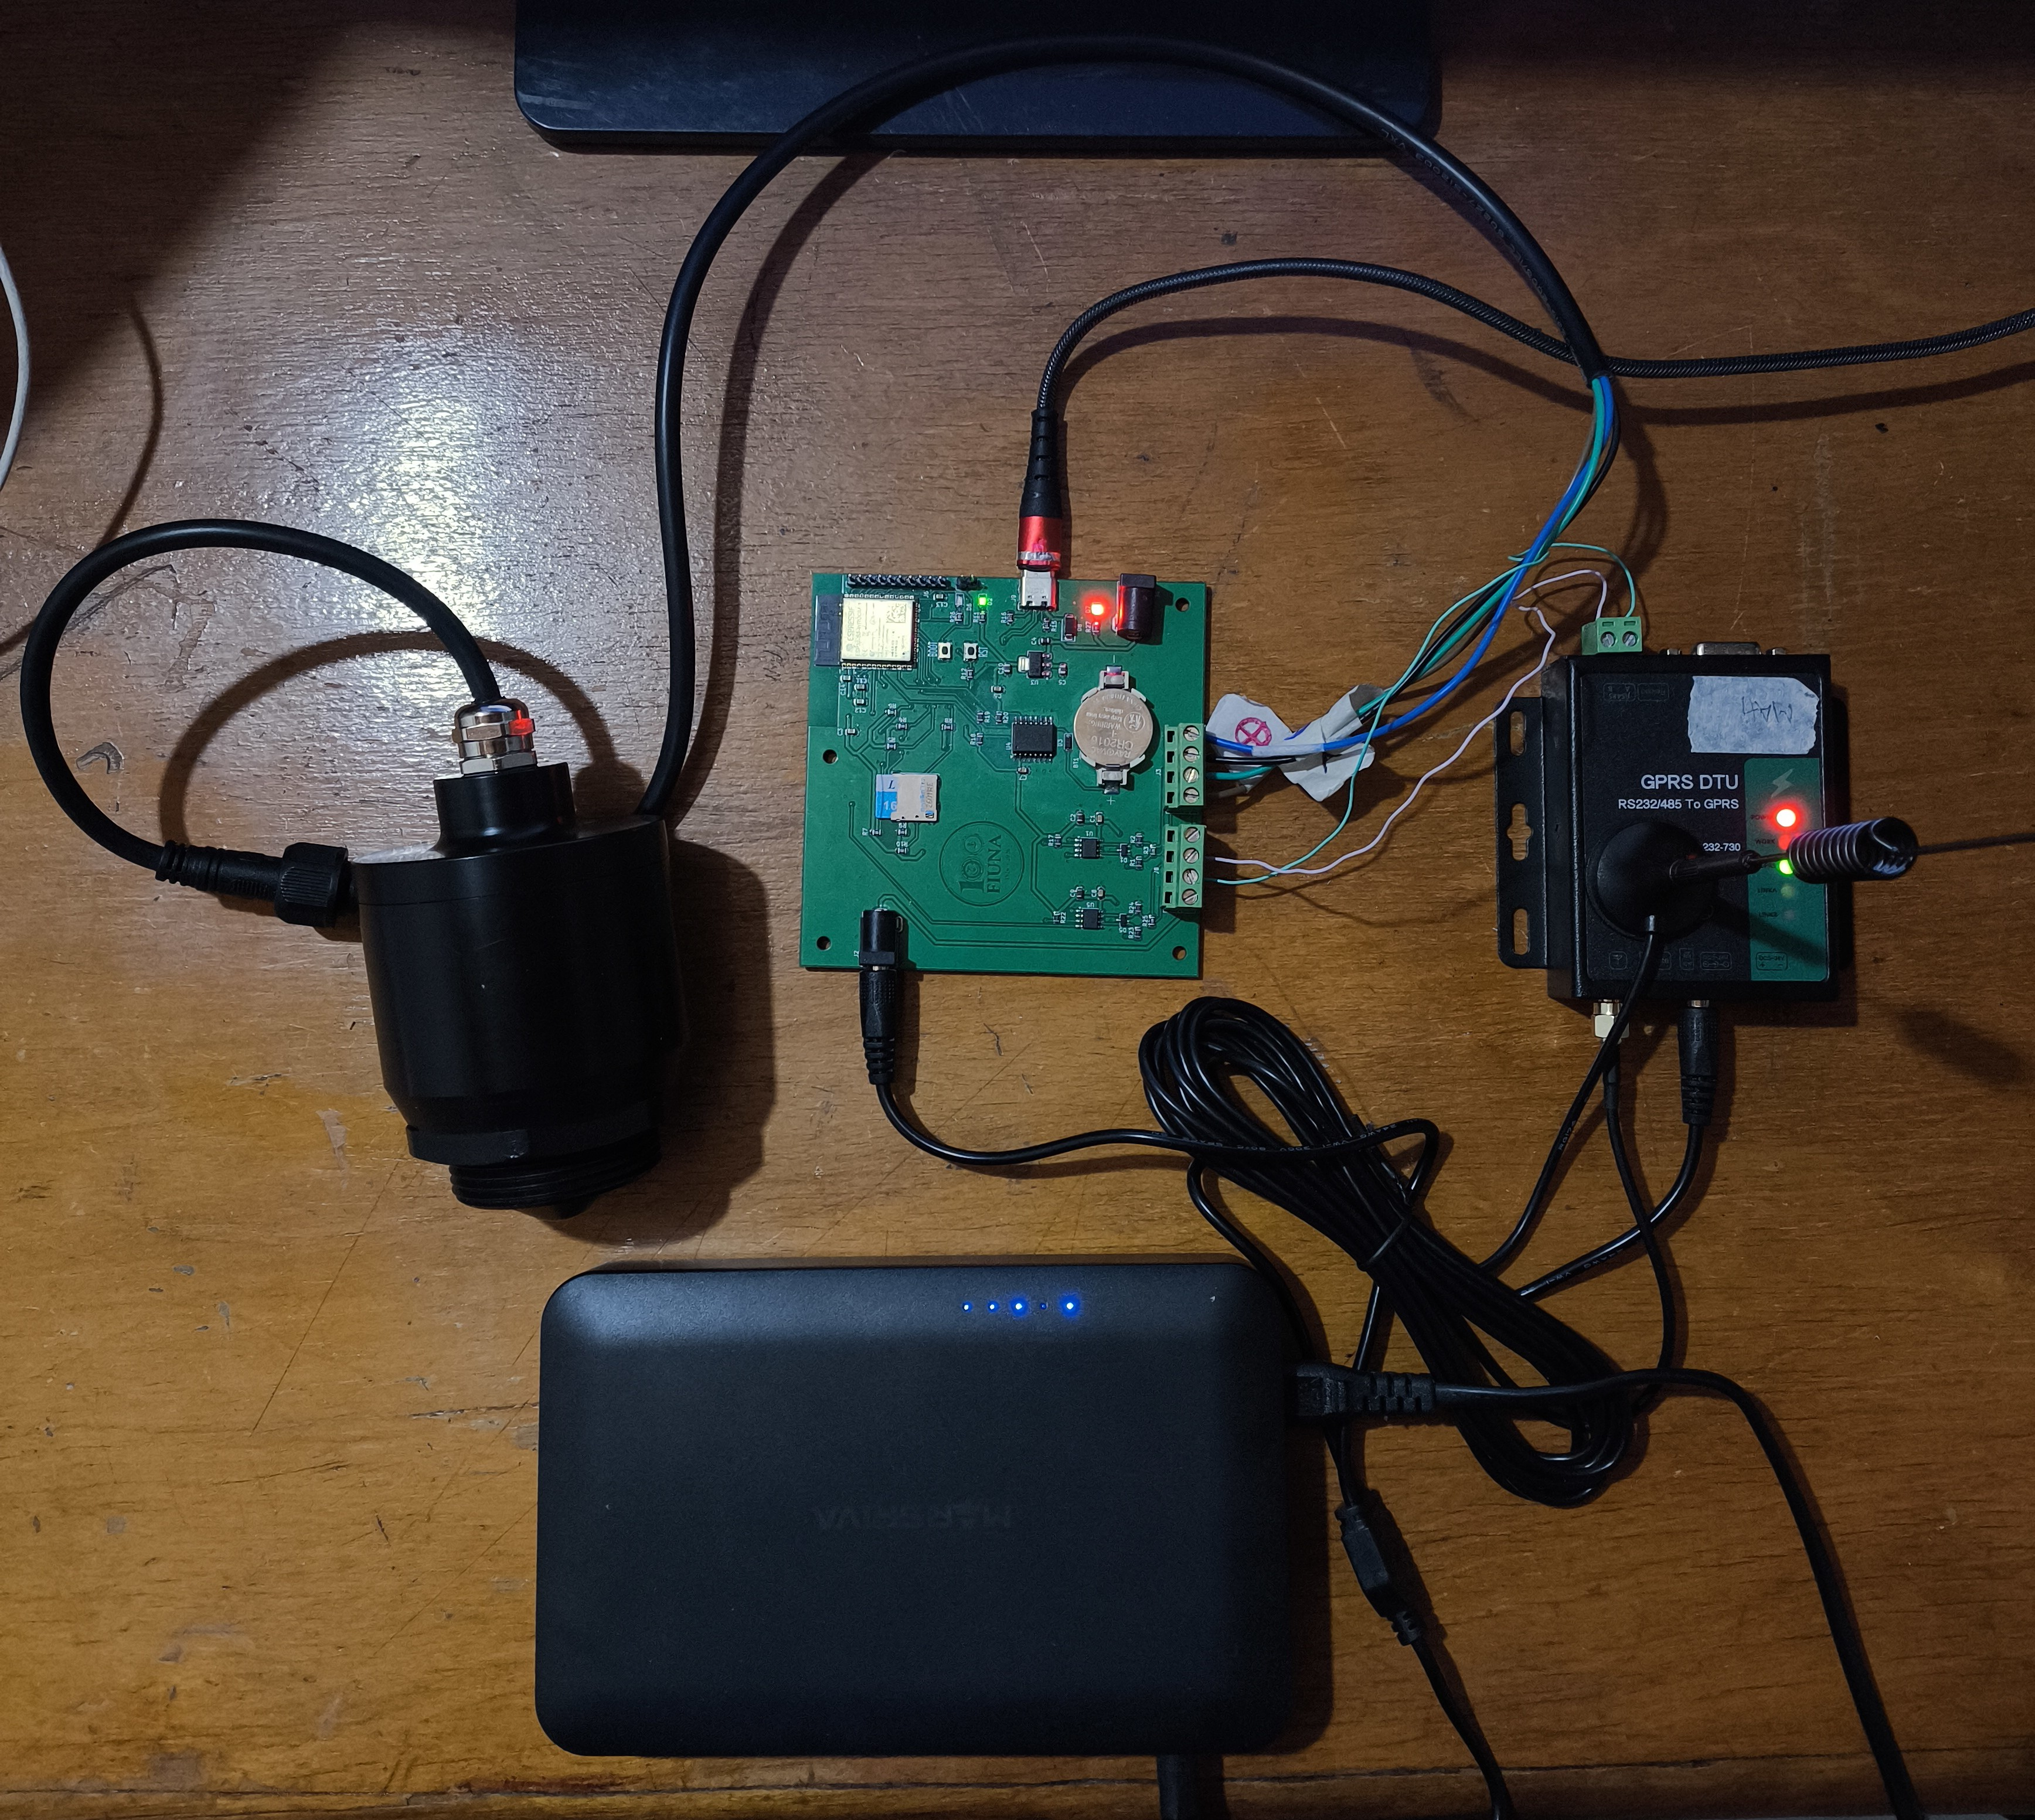
\includegraphics[width=\textwidth]{montaje_p3.jpg}
    \end{minipage}\hfill
    \begin{minipage}[c]{0.48\textwidth}
        \centering
        \small
        \begin{tabular}{lr}
            \toprule
            \textbf{Dato} & \textbf{Valor} \\
            \midrule
            Radar (ficha)       & 1,6--1,9 W \\
            Módem y ESP32       & a medir \\
            Total estimado      & 3--5 W \\
            Batería UPS$^{*}$   & $\approx$ 59 Wh \\
            Autonomía estimada  & 9--15 h \\
            \bottomrule
        \end{tabular}\\[4pt]
        {\footnotesize $^{*}$ 16\,000 mAh a 3,7 V; 80\,\% de eficiencia.}
    \end{minipage}
    \caption{Sistema de P3 con la UPS (izq.) y balance de energía estimado,
    a confirmar midiendo (der.).}
\end{figure}

\needspace{14\baselineskip}
\textbf{Peso de cada dato y capacidad de la SD.} Cada lectura se guarda como
una línea de texto (CSV). Se mide \textbf{cada 5 min}, lo que da \textbf{288 lecturas por día}.

\begin{table}[H]
    \centering
    \caption{Tamaño de cada lectura y lecturas que entran en la SD.}
    \begin{tabular}{lcc}
        \toprule
                               & \textbf{Actual (P3)} & \textbf{Nueva (con id)} \\
        \midrule
        Línea guardada         & \footnotesize\texttt{1780000000,1.234}
                               & \footnotesize\texttt{1780000000,123456,1.234,0.350,0} \\
        Tamaño por lectura     & 17 B (136 bits) & 32 B (256 bits) \\
        Por día (288 lecturas) & 4,9 kB & 9,2 kB \\
        Por año                & 1,8 MB & 3,4 MB \\
        \midrule
        Lecturas en 32 GB      & $\approx 1\,900$ millones & $\approx 1\,000$ millones \\
        Lecturas en 64 GB      & $\approx 3\,800$ millones & $\approx 2\,000$ millones \\
        \bottomrule
    \end{tabular}
\end{table}

Aun con la trama nueva, una SD de 32 GB alcanza para miles de años de
lecturas, así que \textbf{la capacidad no es el límite}. El límite práctico es
el tamaño máximo de un archivo en FAT32 (4 GB), que se alcanzaría recién en unos
1\,300 años. El \textbf{respaldo externo} se hace por seguridad (falla o robo
de la tarjeta), no por falta de espacio: proponemos descargar la SD una vez por
mes, lo que son unos 0,28 MB de datos. La transmisión al servidor también es
liviana: unos 0,3 MB por mes sin contar la sobrecarga del protocolo GPRS.

% ======================================================
% 6. DISENO MECANICO
% ======================================================
\punto{Diseño mecánico/estructural}{3,5}{\SEG\ \FUERA}

\begin{debilidad}
Faltan materiales/tolerancias completos y verificación del soporte, corrosión y
sellado tras mecanizado.
\end{debilidad}

\textbf{Respuesta.}
\begin{itemize}
    \item \SEG\ \textbf{Montaje del sensor:} el radar se monta con su
        \textbf{kit comercial} (soporte orientable, placa para poste y
        3 abrazaderas de acero inoxidable) en el banco de laboratorio, con la
        antena nivelada. Se especifican los materiales del kit y del gabinete,
        y cómo entran los cables. Se presenta foto y plano del banco.
    \item \FUERA\ \textbf{Cálculo por viento, corrosión en sitio y prueba de
        ingreso de agua:} corresponden a la instalación en el arroyo, que
        depende del Departamento de Mecánica y Energía. No se diseña un soporte
        nuevo: se usa el del fabricante.
\end{itemize}

\begin{figure}[H]
    \centering
    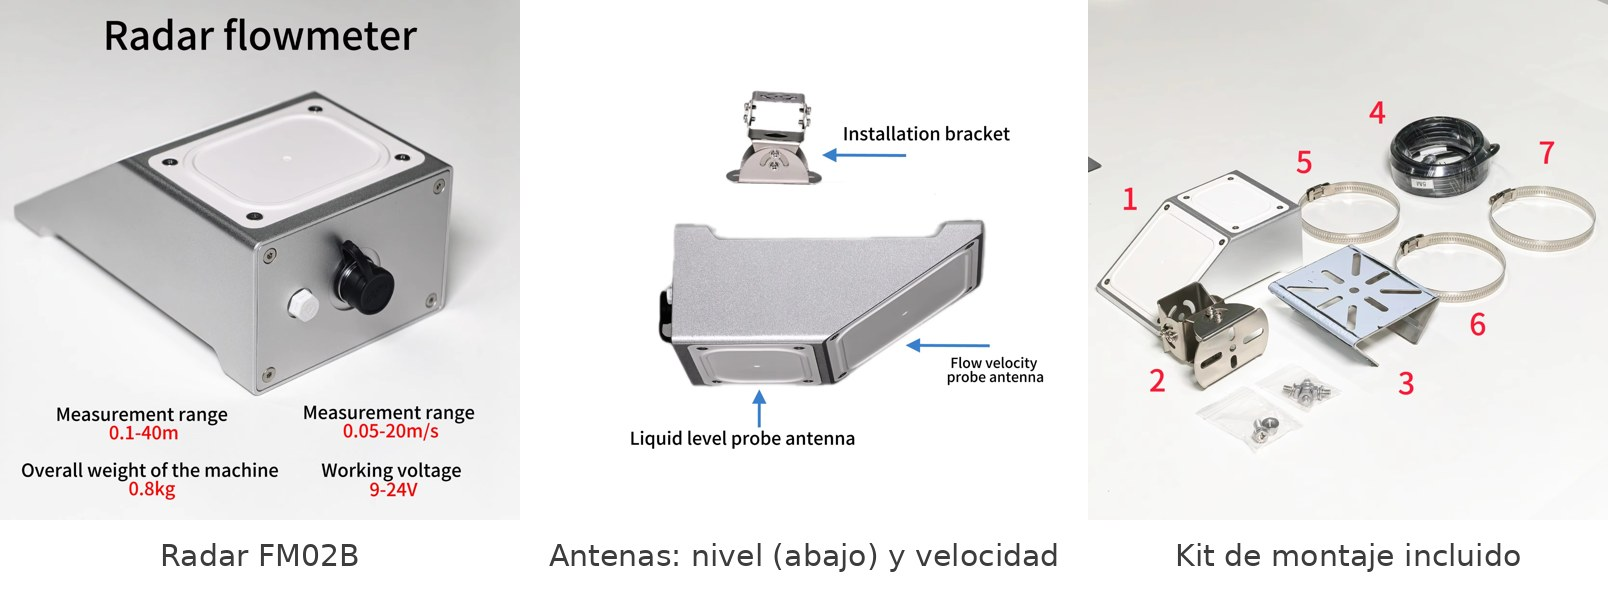
\includegraphics[width=0.9\textwidth]{sensor_fotos.jpg}
    \caption{Radar FM02B y su kit de montaje.}
\end{figure}

% ======================================================
% 7. INTERFAZ DE USUARIO
% ======================================================
\punto{Interfaz de usuario}{4}{\SEG\ \FUERA}

\begin{debilidad}
No queda delimitado qué parte de la plataforma y predicción es contribución
propia; falta tratamiento de dato viejo o inválido.
\end{debilidad}

\textbf{Respuesta.}
\begin{itemize}
    \item \textbf{Aporte delimitado:} la web MburicaoCastAI es del grupo de
        investigación y en el informe solo se cita. El modelo de predicción
        tampoco forma parte de este proyecto académico.
    \item \SEG\ \textbf{Web propia:} hacemos una web para mostrar los datos.
        Primero la probamos con la base de datos histórica de P3 y, cuando el
        radar publique, pasa a mostrar los datos nuevos.
    \item \SEG\ \textbf{Dato viejo o inválido:} la web muestra la antigüedad de
        la última lectura (aviso si pasan más de 15 min sin datos, es decir, 3 lecturas) y el estado
        del sensor (campo \emph{estado} de la trama).
    \item \FUERA\ \textbf{Usuarios y permisos:} los datos son abiertos y la web
        solo muestra información; no hay nada que restringir.
\end{itemize}

\begin{figure}[H]
    \centering
    \resizebox{0.95\textwidth}{!}{% Boceto de la web propia (valores ilustrativos)
\begin{tikzpicture}[
    tarjeta/.style={draw=gray!50, fill=white, rounded corners=3pt, minimum height=1.35cm, align=center, font=\small},
    rotulo/.style={font=\scriptsize, text=gray!60!black}
]
    % Ventana del navegador
    \draw[gray!60, fill=gray!5, rounded corners=5pt] (0,0) rectangle (13,7.6);
    \fill[gray!25, rounded corners=5pt] (0,7.0) rectangle (13,7.6);
    \fill[gray!25] (0,7.0) rectangle (13,7.2);
    \foreach \x in {0.3,0.6,0.9} \fill[gray!55] (\x,7.3) circle (0.08);
    \node[anchor=west, font=\small\bfseries] at (1.3,7.3) {Estación de nivel -- arroyo Mburicaó (datos abiertos)};

    % Alarma
    \draw[draw=orange!80!black, fill=orange!15, rounded corners=3pt] (0.4,6.15) rectangle (12.6,6.75);
    \node[font=\small, text=orange!50!black] at (6.5,6.45) {\textbf{Alarma:} el nivel superó el umbral configurado};

    % Tarjetas
    \node[tarjeta, minimum width=2.8cm] at (1.85,5.1) {{\scriptsize\color{gray!60!black} Nivel actual}\\{\Large\bfseries 0,52 m}};
    \node[tarjeta, minimum width=2.8cm] at (4.95,5.1) {{\scriptsize\color{gray!60!black} Velocidad}\\{\Large\bfseries 0,35 m/s}};
    \node[tarjeta, minimum width=2.8cm] at (8.05,5.1) {{\scriptsize\color{gray!60!black} Última lectura}\\{\bfseries hace 2 min}};
    \node[tarjeta, minimum width=2.8cm] at (11.15,5.1) {{\scriptsize\color{gray!60!black} Estado del sensor}\\{\bfseries\textcolor{agua!80!black}{$\bullet$ OK}}};

    % Gráfico de históricos
    \draw[gray!50, fill=white, rounded corners=3pt] (0.4,0.4) rectangle (12.6,4.1);
    \node[anchor=west, font=\footnotesize\bfseries] at (0.6,3.8) {Históricos};
    \node[anchor=east, rotulo] at (12.4,3.8) {24 h \quad 7 días \quad 30 días};
    \draw[gray!40] (1,0.8) -- (12.2,0.8);
    \draw[gray!40] (1,0.8) -- (1,3.4);
    \draw[radar, thick] plot[smooth] coordinates {(1,1.1) (2,1.15) (3,1.1) (4,1.2) (4.6,2.9) (5.1,1.5) (6,1.2) (7,1.15) (8,1.2) (8.6,2.3) (9.1,1.3) (10,1.15) (11,1.2) (12.2,1.15)};
    \draw[orange!80!black, dashed] (1,2.6) -- (12.2,2.6) node[above left, rotulo, text=orange!60!black] {umbral de alarma};
\end{tikzpicture}
}
    \caption{Boceto de la web propia (valores ilustrativos).}
\end{figure}

% ======================================================
% 8. VALIDACION Y SEGURIDAD
% ======================================================
\punto{Validación y seguridad}{2,5}{\SEG\ \FUERA}
\label{sec:validacion}

\begin{debilidad}
La existencia de microSD no prueba ausencia de pérdidas/duplicados ni exactitud
de medición.
\end{debilidad}

\textbf{Respuesta.} Es el centro del segundo parcial. En P3 las pruebas se
mostraron con video; ahora se cuantifican. Las cantidades son un mínimo
propuesto y se ajustan al montar el banco. Los cortes, la disponibilidad y la
autonomía no dependen del sensor, así que se ensayan con el sensor de P3
mientras llega el radar (primera o segunda semana de noviembre).

\begin{table}[H]
    \centering
    \caption{Ensayos en banco de laboratorio.}
    \begin{tabularx}{\textwidth}{>{\raggedright\arraybackslash}p{2.3cm}LL>{\raggedright\arraybackslash}p{2.1cm}}
        \toprule
        \textbf{Ensayo} & \textbf{Cómo} & \textbf{Qué se reporta} &
            \textbf{Umbral} \\
        \midrule
        Exactitud & Radar sobre un recipiente con agua; $\geq$ 4 alturas
            $\times$ 10 lecturas, frente a cinta métrica. & Error medio y
            máximo (mm). & $\leq \pm$10 mm \\
        Cortes de red & $\geq$ 10 cortes del módem o del servidor, en distintos
            momentos. & Perdidos y duplicados (cruce de id entre SD y
            servidor); tiempo de recuperación. & 0 perdidos, 0 duplicados \\
        Cortes de energía & $\geq$ 10 cortes, incluso durante la escritura en
            SD y el envío. & Lo anterior + integridad de la SD. & 0 perdidos,
            0 duplicados \\
        Disponibilidad & 7 días continuos. & \% de datos recibidos. &
            $\geq$ 95\,\% \\
        Autonomía & Corte de red con la UPS cargada. & Horas hasta el
            apagado. & Se informa \\
        \bottomrule
    \end{tabularx}
\end{table}

\begin{minipage}[c]{0.5\textwidth}
\textbf{Por qué hace falta el id.} Hoy el id lo asigna el servidor, así que
un hueco en los datos no dice si la estación dejó de medir o si el dato se
perdió en el camino. Con el id generado por la estación, cada hueco se puede
explicar.

\medskip
En la captura, entre las 00:28 y las 01:54 no hay datos, y desde el servidor
no se puede saber por qué.
\end{minipage}\hfill
\begin{minipage}[c]{0.46\textwidth}
    \centering
    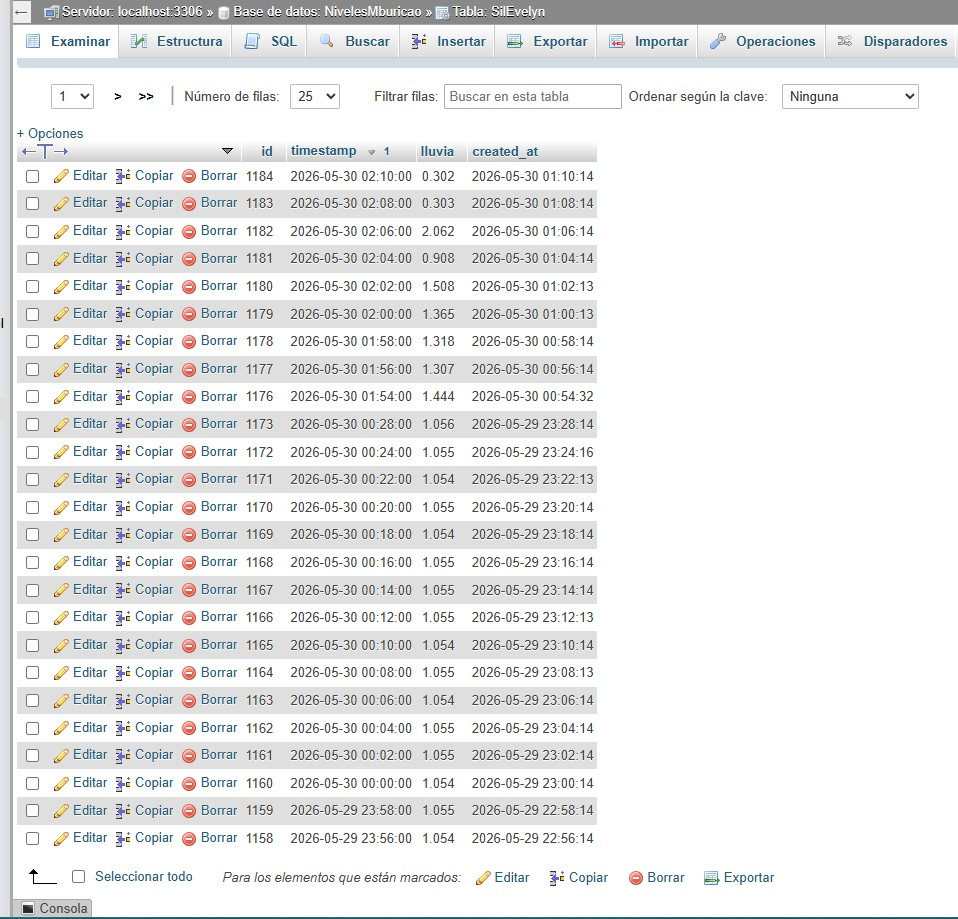
\includegraphics[width=\textwidth]{base_datos.jpg}
    \captionof{figure}{Registros del servidor en P3.}
\end{minipage}

\textbf{Cuidado con el recipiente.} El haz del radar se abre 14°: a 1 m cubre
un círculo de 25 cm y a 2 m, de 49 cm. Con un balde común ($\approx$ 30 cm)
se mide hasta $\approx$ 1 m; para llegar a 2 m hace falta un recipiente más
ancho, o el haz toca los bordes y da lecturas falsas.

\begin{figure}[H]
    \centering
    \resizebox{!}{7cm}{% Haz de 14 grados del radar sobre un balde de 30 cm (escala: 1 m = 4 cm)
% Superficie del agua en y = 1.2; borde del balde en y = 1.4; medio ancho del balde 0.6
\begin{tikzpicture}[
    balde/.style={draw=gray!70!black, very thick},
    sensor/.style={fill=gray!70!black, minimum width=0.6cm, minimum height=0.35cm, inner sep=0pt},
    cota/.style={<->, >=Stealth, gray!60!black},
    rotulo/.style={font=\footnotesize, align=center}
]
    % ---------- Caso 1: sensor a 1 m del agua ----------
    \begin{scope}
        \fill[agua!25] (-0.6,0) rectangle (0.6,1.2);
        \draw[balde] (-0.6,1.4) -- (-0.6,0) -- (0.6,0) -- (0.6,1.4);
        \fill[radar!25] (0,5.2) -- (-0.49,1.2) -- (0.49,1.2) -- cycle;
        \draw[radar, thick] (-0.49,1.2) -- (0,5.2) -- (0.49,1.2);
        \node[sensor] at (0,5.38) {};
        \draw[cota] (1.0,5.2) -- node[right, rotulo] {1 m} (1.0,1.2);
        \node[rotulo, below] at (0,-0.15) {Haz de 25 cm\\\textcolor{agua!80!black}{\textbf{entra en el balde}}};
    \end{scope}

    % ---------- Caso 2: sensor a 2 m del agua ----------
    \begin{scope}[xshift=5cm]
        \fill[agua!25] (-0.6,0) rectangle (0.6,1.2);
        \draw[balde] (-0.6,1.4) -- (-0.6,0) -- (0.6,0) -- (0.6,1.4);
        \fill[radar!25] (0,9.2) -- (-0.98,1.2) -- (0.98,1.2) -- cycle;
        \draw[radar, thick] (-0.98,1.2) -- (0,9.2) -- (0.98,1.2);
        \node[sensor] at (0,9.38) {};
        \fill[red] (-0.6,1.4) circle (2.2pt) (0.6,1.4) circle (2.2pt);
        \draw[cota] (1.5,9.2) -- node[right, rotulo] {2 m} (1.5,1.2);
        \node[rotulo, below] at (0,-0.15) {Haz de 49 cm\\\textcolor{red!80!black}{\textbf{toca los bordes}}};
    \end{scope}

    % Ángulo del haz
    \node[rotulo, radar] at (5,9.95) {14°};
\end{tikzpicture}
}
    \caption{Haz de 14° sobre un balde de 30 cm, con el sensor a 1 m y a 2 m.}
\end{figure}

\FUERA\ \textbf{Calibrar todo el rango del radar (0,1--40 m):} el laboratorio
permite como máximo 1 a 2 m de altura.

% ======================================================
% 9. BIBLIOGRAFIA Y APORTE PROPIO
% ======================================================
\punto{Bibliografía y aporte propio}{3,5}{\SEG}

\begin{debilidad}
Estado del arte centrado en componentes; sensor referido por enlace comercial
sin identificación metrológica suficiente.
\end{debilidad}

\textbf{Respuesta.}
\begin{itemize}
    \item \textbf{Sensor:} se cita el manual oficial del radar (Luda / POLIVIR
        FM02B, part number LDFM04\_B) con fabricante, modelo y versión del
        documento. Se pide al fabricante o se toma del manual que trae el
        equipo. También hace falta para el firmware: la ficha comercial no
        trae el protocolo RS485.
    \item \textbf{Sistemas completos:} los profesores del área de hidrología
        del proyecto cuentan con otros sistemas de medición de nivel. Los
        describimos en el estado del arte y los usamos como comparación.
    \item \textbf{Atribución:} Grafana, la web MburicaoCastAI y el modelo de
        predicción se citan como trabajos externos a este proyecto.
\end{itemize}

% ======================================================
% 10. VIABILIDAD Y DOCUMENTACION
% ======================================================
\punto{Viabilidad y documentación}{3,5}{\SEG\ \FUERA}

\begin{debilidad}
Resumen dice que CAD queda pendiente aunque existen planos; faltan costos
mecánicos y recurrentes claramente integrados.
\end{debilidad}

\textbf{Respuesta.}
\begin{itemize}
    \item \SEG\ \textbf{Documento:} se corrige el resumen (los planos existen).
    \item \SEG\ \textbf{Costos:} lista de materiales completa: PCB y
        componentes, radar (USD 690,41 + 64,80 de envío), kit de montaje,
        gabinete, UPS y módem. El costo recurrente es el plan mensual de datos
        del módem, que paga la Facultad.
    \item \SEG\ \textbf{Cronograma:} semanal hasta el segundo parcial (figura
        siguiente). El radar llega entre la primera y la segunda semana de
        noviembre, así que las pruebas que no dependen del sensor (cortes,
        disponibilidad y autonomía) se hacen antes con el sensor de P3. Con el
        radar quedan su firmware, el montaje en banco y la exactitud.
    \item \FUERA\ \textbf{Cronograma de instalación y piloto en el arroyo:}
        depende del Departamento de Mecánica y Energía.
\end{itemize}

\begin{figure}[H]
    \centering
    \resizebox{\textwidth}{!}{% Cronograma hasta el segundo parcial (16/11/2026), por semanas
\begin{ganttchart}[
    hgrid, vgrid,
    x unit=2.5cm, y unit chart=0.6cm, y unit title=0.6cm,
    title label font=\footnotesize\bfseries,
    bar label font=\footnotesize,
    milestone label font=\footnotesize\bfseries,
    bar/.append style={fill=radar!60, draw=radar},
    milestone/.append style={fill=agua, draw=agua},
    group/.append style={fill=gray!60},
]{1}{5}
    \gantttitle{12--18 oct}{1}
    \gantttitle{19--25 oct}{1}
    \gantttitle{26 oct--1 nov}{1}
    \gantttitle{2--8 nov}{1}
    \gantttitle{9--15 nov}{1} \\
    \ganttbar{Manual del radar, comparación, BOM}{1}{1} \\
    \ganttbar{Disponibilidad de los datos de P3}{1}{1} \\
    \ganttbar{Firmware radar + trama + SD}{2}{3} \\
    \ganttbar{Servidor (trama nueva)}{2}{2} \\
    \ganttbar{Web propia}{2}{4} \\
    \ganttbar{Montaje en banco}{3}{3} \\
    \ganttbar{Exactitud y consumo}{3}{3} \\
    \ganttbar{Cortes, autonomía, 7 días}{4}{4} \\
    \ganttbar{Informe del 2.\textsuperscript{o} parcial}{5}{5} \\
    \ganttmilestone{Entrega: 16/11}{5}
\end{ganttchart}
}
    \caption{Cronograma hasta la entrega del 16 de noviembre de 2026.}
\end{figure}

% ======================================================
% FUERA DE ALCANCE
% ======================================================
\needspace{12\baselineskip}
\section*{Resumen de puntos fuera de alcance}

\begin{table}[H]
    \centering
    \begin{tabularx}{\textwidth}{>{\raggedright\arraybackslash}p{4.6cm}L}
        \toprule
        \textbf{Punto} & \textbf{Justificación} \\
        \midrule
        Piloto e instalación en el arroyo & Depende del Departamento de
            Mecánica y Energía. Se reemplaza por un banco de laboratorio. \\
        Viento, corrosión y prueba de ingreso de agua & Son propios de la
            instalación en el sitio; se usa el kit comercial del fabricante. \\
        Calibrar en todo el rango (0,1--40 m) & El laboratorio permite hasta
            1--2 m de altura. \\
        Usuarios y permisos en la web & Los datos son abiertos; la web solo
            muestra información. \\
        Web MburicaoCastAI y modelo de predicción & No forman parte de este
            proyecto académico; solo se citan. \\
        \bottomrule
    \end{tabularx}
\end{table}

\end{document}
